% Source: AESP_466_ClassWork/Supplements/Notes/latex/6.6.3/6.6.3.tex

\documentclass[border=4pt]{standalone}
\usepackage{amsmath,amssymb,amsthm}
\usepackage{graphicx}
\usepackage{tikz}
\usepackage{xcolor}
\usetikzlibrary{arrows.meta,calc,positioning,decorations.markings,patterns,shapes.geometric,angles,quotes}

\definecolor{Garnet}{HTML}{73000A}
\definecolor{USC_Rose}{HTML}{CC2E40}
\definecolor{USC_Blue}{HTML}{466A9F}
\definecolor{USC_Slate}{HTML}{1F414D}
\definecolor{USC_Olive}{HTML}{65780B}
\definecolor{USC_Lime}{HTML}{CED318}
\definecolor{USC_Gold}{HTML}{A49137}
\definecolor{USC_Black90}{HTML}{565556}
\definecolor{USC_Black10}{HTML}{ECECEC}

\newcommand{\vect}[1]{\mathbf{#1}}
\newcommand{\mat}[1]{\mathbf{#1}}
\newcommand{\uvec}[1]{\hat{\mathbf{#1}}}
\newcommand{\transpose}{^{\mkern-1.5mu\mathsf{T}}}
\newcommand{\inv}{^{-1}}
\newcommand{\deriv}[2]{\frac{d #1}{d #2}}
\newcommand{\pderiv}[2]{\frac{\partial #1}{\partial #2}}

\begin{document}
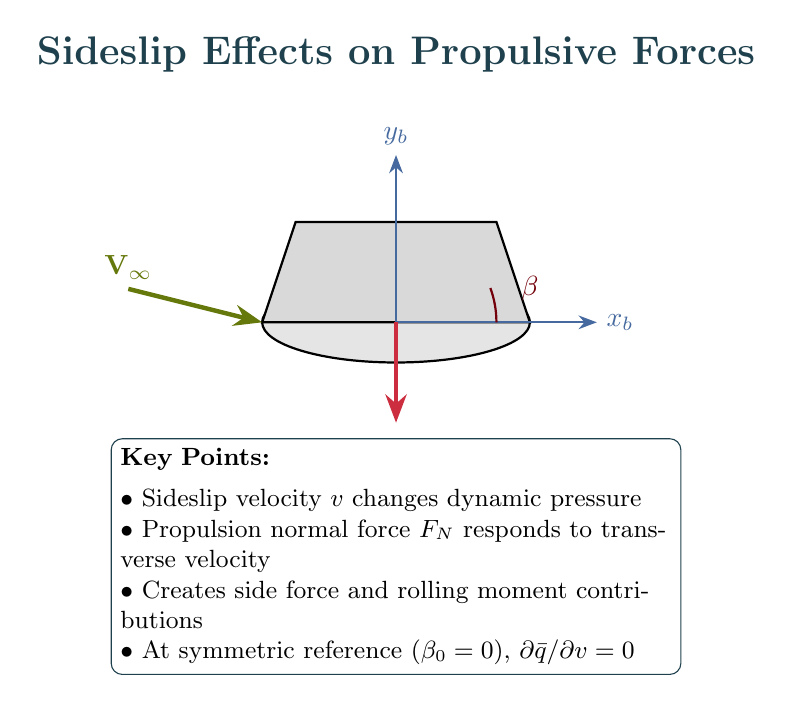
\begin{tikzpicture}[>=Stealth, scale=0.85]
    % Title
    \node[font=\Large\bfseries, USC_Slate] at (5,6) {Sideslip Effects on Propulsive Forces};

    % Aircraft top view
    \draw[thick, fill=gray!20] (5,2) ellipse (2 and 0.6);
    \draw[thick, fill=gray!30] (3,2) -- (3.5,3.5) -- (6.5,3.5) -- (7,2) -- cycle; % wing

    % Velocity vector (with sideslip)
    \draw[->, ultra thick, USC_Olive] (1,2.5) -- (3,2);
    \node[USC_Olive, above left] at (1.5,2.5) {$\mathbf{V}_\infty$};

    % Body x-axis
    \draw[->, thick, USC_Blue] (5,2) -- (8,2);
    \node[USC_Blue, right] at (8,2) {$x_b$};

    % Body y-axis
    \draw[->, thick, USC_Blue] (5,2) -- (5,4.5);
    \node[USC_Blue, above] at (5,4.5) {$y_b$};

    % Sideslip angle
    \draw[thick, Garnet] (6.5,2) arc (0:20:1.5);
    \node[Garnet] at (7,2.5) {$\beta$};

    % Normal force from propulsion
    \draw[->, ultra thick, USC_Rose] (5,2) -- (5,0.5);
    \node[USC_Rose, below] at (5,0.3) {$F_N$};

    % Annotation
    \node[draw=USC_Slate, fill=white, rounded corners, align=left, font=\small, text width=7cm] at (5,-1.5) {
        \textbf{Key Points:}\\[4pt]
        $\bullet$ Sideslip velocity $v$ changes dynamic pressure\\
        $\bullet$ Propulsion normal force $F_N$ responds to transverse velocity\\
        $\bullet$ Creates side force and rolling moment contributions\\
        $\bullet$ At symmetric reference ($\beta_0 = 0$), $\partial\bar{q}/\partial v = 0$
    };

\end{tikzpicture}
\end{document}
